\chapter{CFA Level 1}
This is a very brief note for the CFA level 1 which has been made during my study for this examination.


\section{QM - The Time Value of Money}
The Time Value of Money (TVM) procedures imply \textbf{compound interest} and \textbf{interest on interest}. TVM applications call for determining the \textbf{future value} $FV$ or the \textbf{present value} $PV$ of an investment's cash flows as a result of the effects of compound interest. 
\begin{itemize}
	\setlength\itemsep{0em}
	\item $FV$: projecting the cash flows forward to the end of the investment's life;
	\item $PV$: bringing the cash flows from an investment back to the beginning of the investment's life.		
\end{itemize}

To solve a TVM problem, it is often a good idea to draw a \textbf{time line} - a diagram of the cash flows associated with that TVM problem. Cash outflows (payments) are given a negative sign, and cash inflows (receipts) are given a positive sign. Figure below illustrates a time line for an investment that cost \$1000 today (outflow) and will return a stream of cash payments (inflows) of \$300 per year at the end of each of the next five years.

\newcommand{\tvma}{{"-1000","+300","+300","+300","+300","+300"}}
\begin{center}
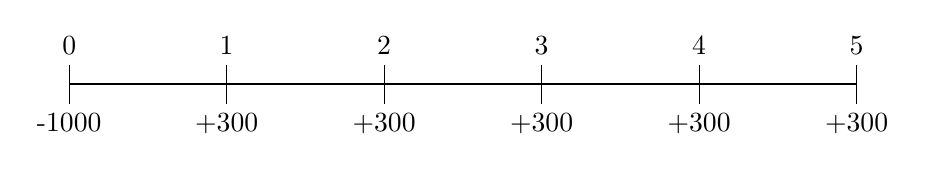
\begin{tikzpicture}
    \draw[thick] (0,0) -- (10,0);
    \foreach \x [count=\k] in {0,...,5}
        {
        \draw[thin] (\x*2, -0.25) -- (\x*2, 0.25);
        \node[above] at (\x*2, 0.25) {\pgfmathparse{\x}\pgfmathresult};
        \node[below] at (\x*2, -0.25) {\pgfmathparse{\tvma[\k-1]}\pgfmathresult};
        }
\end{tikzpicture}
\end{center}

Please recognize that the cash flows occur at the end of the period depicted on the time line, and the end of one period is the same as the beginning of the next period. 



\subsection{Interest rates}

\subsubsection{Introduction}
Interest rates are the measure of the TVM, although risk differences in financial securities lead to different views in their equilibrium interest rates. 
\begin{itemize}
	\setlength\itemsep{0em}
	\item \textbf{Required rate of return}: for a particular investment of an investor or a lender;
	\item \textbf{Discount rates}: when an individual borrow funds;
	\item \textbf{Opportunity cost} of current consumption: the opportunity forgone when current consumption is chosen rather than saving. 
\end{itemize}

Components of the interest rate can be broken down into:
\begin{align*}
    \text{required interest rate on a security } &=  \text{real risk-free rate} \\
      &+ \text{expected inflation rate}\\
      &+ \text{default risk premium}   \\
      &+ \text{liquidity premium}      \\
      &+ \text{maturity risk premimum} 
\end{align*}
\begin{itemize}
	\setlength\itemsep{0em}
	\item \textbf{real risk-free rate}: a theoretical rate on a single-period loan that has no expectation of inflation;
	\item \textbf{default risk}: a borrower may not make the promised payments in a timely manner;
	\item \textbf{liquidity risk}: an investment, when is sold for cash quickly, may worth less than its fair value;
	\item \textbf{maturity risk}: longer term bonds have more maturity risk than shorter term bonds since they are more volatile. 
\end{itemize}



\subsubsection{Effective annual rate/yield}
Financial institutions usually quote rates as stated annual interest rates, along with a compounding frequency. The rate of interest that investors actually realize as a result of compounding is known as the \textbf{effective annual rate} (EAR) or \textbf{effective annual yield} (EAY). EAR represents the annual rate of return actually being earned after adjustments have been made for different compounding periods.
\begin{equation}
	\text{EAR} = (1 + r_p)^m - 1
\end{equation}
in which $r_p$ is the \textbf{periodic rate} - the rate of interest earned over a single compounding period which is equal to the stated annual rate over the number of compounding periods per year $m$. For example, the EARs for a stated rate of 6\% compounded semi-annually, quarterly and daily can be computed as follows:
\begin{align*}
	\text{semi-annually: } & \left( 1 + \frac{6\%}{2} \right)^2 - 1     = 6.090\% \\
	\text{quarterly: }     & \left( 1 + \frac{6\%}{4} \right)^4 - 1     = 6.136\% \\
	\text{daily: }         & \left( 1 + \frac{6\%}{365} \right)^{365} - 1 = 6.183\% 
\end{align*}



\subsection{A single cash flow}
In this section, we will study for how compute the future value $FV$ and present value $PV$ of a single cash flow. Future value is the amount to which a current deposit will grow over time when it is placed in an account paying compound interest. For a single cash flow, we have:
\begin{equation}
    FV_{N} = PV (1 + r)^{N} \quad\quad PV = FV_{N} (1 + r)^{-N}
\end{equation}
in which: $PV$ is the amount of money invested today (the present value), $r$ the rate of return per compounding period, $N$ the total number of compounding period. 

\newcommand{\timb}{{"0","1","...","N-1","N"}}
\newcommand{\tvmb}{{"$PV$","","","","$FV = PV(1 + r)^{N}$"}}
\begin{center}
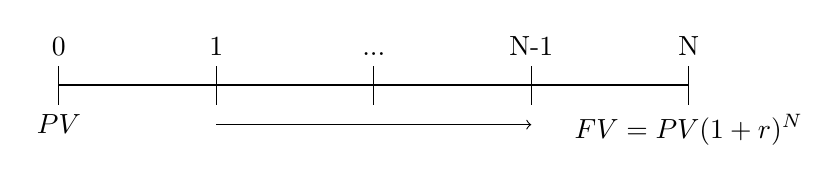
\begin{tikzpicture}
    \draw[thick] (0,0) -- (8,0);
    \foreach \x [count=\k] in {0,...,4}
        {
        \draw[thin] (\x*2, -0.25) -- (\x*2, 0.25);
        \node[above] at (\x*2, 0.25)  {\pgfmathparse{\timb[\k-1]}\pgfmathresult};
        \node[below] at (\x*2, -0.25) {\pgfmathparse{\tvmb[\k-1]}\pgfmathresult};
        }
    \draw (2, -0.5) edge[->] (6, -0.5);
\end{tikzpicture}
\end{center}


For the investments paying interest more than once a year, financial institutions often quote an annual interest rate that we refer as the \textbf{stated annual interest rate} or \textbf{quoted interest rate}, denoted by $r_s$. Then the future value is computed as:
\begin{equation}
	FV_{N} = PV \left( 1 + \frac{r_s}{m} \right)^{mN} \quad\quad PV = FV_{N} \left( 1 + \frac{r_s}{m} \right)^{-mN}
\end{equation}
with $m$ is the number of compounding per year and $N$ is the number of years. 

When the compounding is continuous, i.e. the number of compounding periods per year becomes infinite or $m \rightarrow \infty$, we have:
\begin{equation}
	FV_{N} = PV e^{r_s N} \quad\quad PV = FV_{N} e^{-r_s N}
\end{equation}
with the constant $e \approx 2.71828$.


\subsection{A series of cash flows}
An \textbf{annuity} is a finite set of level sequential cash flows (CFs), i.e. equal cash flows occurs at equal intervals over a given period. 
\begin{itemize}
	\setlength\itemsep{0em}
	\item \textbf{Ordinary annuities} (OA): cash flows occur at the end of each compounding period;
	\item \textbf{Annuities due} (AD): cash flows occur at the beginning of each period. 
\end{itemize}
Calculating $FV$ and $PV$ of an annuity is not so much different from calculating $FV$ and $PV$ of a single cash flow. 

Let's consider an ordinary annuity that pays $PMT = \$200$ per year at the end of each of the next $N = 4$ years. Given the investment is expected to earn $r (I/Y) = 10\%$ rate of return, then:
\begin{itemize}
	\setlength\itemsep{0em}
	\item $FV$ of this ordinary annuities is given by:
	\begin{equation}
		FV_N = PMT \left[ \frac{(1+r)^N - 1}{r} \right] = 928.20
	\end{equation}
	\item $PV$ of this ordinary annuities is given by:
	\begin{equation}
		PV_0 = PMT \left[ \frac{1 - \frac{1}{(1+r)^N}}{r} \right] = 633.97
	\end{equation}	
\end{itemize}
You can actually use financial calculators to quickly calculate the $FV$ and $PV$ without using these formula. Illustration of this ordinary annuities is given below:
\newcommand{\timc}{{"0","1","2","3","4"}}
\newcommand{\tvmc}{{"","+200","+200","+200","+200"}}
\begin{center}
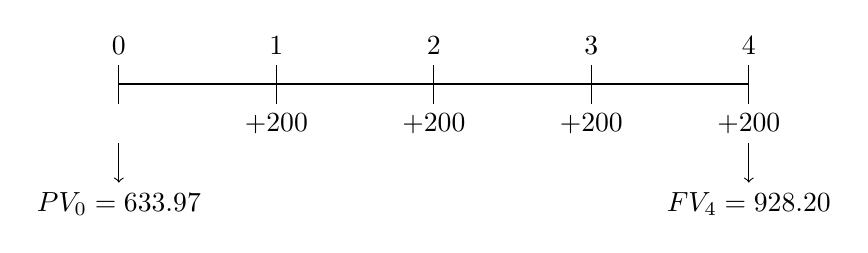
\begin{tikzpicture}
    \draw[thick] (0,0) -- (8,0);
    \foreach \x [count=\k] in {0,...,4}
        {
        \draw[thin] (\x*2, -0.25) -- (\x*2, 0.25);
        \node[above] at (\x*2, 0.25)  {\pgfmathparse{\timc[\k-1]}\pgfmathresult};
        \node[below] at (\x*2, -0.25) {\pgfmathparse{\tvmc[\k-1]}\pgfmathresult};
        }
    \draw (8, -0.75) edge[->] (8, -1.25);
    \node[below] at (8, -1.25) {\pgfmathparse{"$FV_4 = 928.20$"}\pgfmathresult};
    \draw (0, -0.75) edge[->] (0, -1.25);
    \node[below] at (0, -1.25) {\pgfmathparse{"$PV_0 = 633.97$"}\pgfmathresult};    
\end{tikzpicture}
\end{center}
When an ordinary annuity beginning later than $t = 1$, i.e. at the year $T > 1$, first we need to calculate $PV_T$ using the above formula, then $PV_0$ using a basic formula $PV_0 = PV_T (1+r)^{-T}$. This example is illustrated below:
\newcommand{\timd}{{"0","1","2","3","4","5","6"}}
\newcommand{\tvmd}{{"","","","+100","+100","+100","+100"}}
\begin{center}
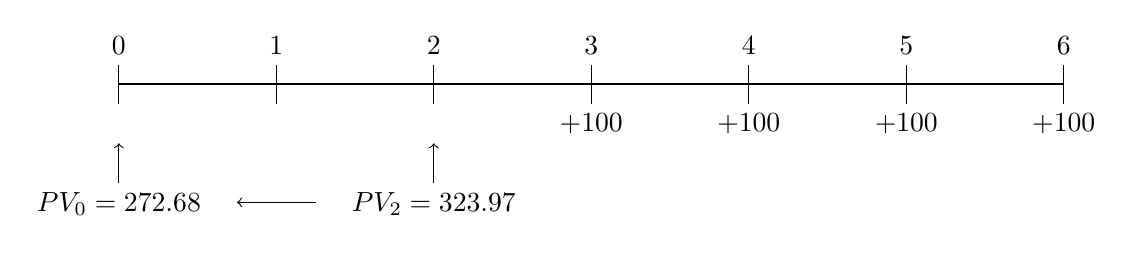
\begin{tikzpicture}
    \draw[thick] (0,0) -- (12,0);
    \foreach \x [count=\k] in {0,...,6}
        {
        \draw[thin] (\x*2, -0.25) -- (\x*2, 0.25);
        \node[above] at (\x*2, 0.25)  {\pgfmathparse{\timd[\k-1]}\pgfmathresult};
        \node[below] at (\x*2, -0.25) {\pgfmathparse{\tvmd[\k-1]}\pgfmathresult};
        }
    \draw (4, -0.75) edge[<-] (4, -1.25);
    \node[below] at (4, -1.25) {\pgfmathparse{"$PV_2 = 323.97$"}\pgfmathresult};
    \draw (0, -0.75) edge[<-] (0, -1.25);
    \node[below] at (0, -1.25) {\pgfmathparse{"$PV_0 = 272.68$"}\pgfmathresult}; 
    \draw (1.5, -1.5) edge[<-] (2.5, -1.5);
\end{tikzpicture}
\end{center}
If a face value is paid at maturity of an investment, this will be added to the final $FV$ at maturity; and from this final value, we can back-calculate the $PV$ of the investment. 

Consider the case of an ordinary annuity that extends indefinitely, called a perpetuity - a perpetual annuity. As long as the interest rates are positive, the $PV$ of a perpetuity can be computed as:
\begin{equation}
	PV = \frac{PMT}{1+r} + \frac{PMT}{1+r^2} + ... = PMT \sum_{i=1}^{\infty} \left[ \frac{1}{(1+r)^i} \right] = \frac{PMT}{r}
\end{equation}

Given the definite of the ordinary annuities and the annuities due, the $FV$ and $PV$ of an annuity due can easily be calculated from those of an ordinary annuity:
\begin{equation}
	FV_{AD} = FV_{OD} (1+r) \quad\quad PV_{AD} = PV_{OD} (1+r)
\end{equation}

In reality, we may encounter a series of uneven cash flow more often then a series of even cash flow. The backbone relationship of $PV$, $FV$, $N$ and $r$ behind is still the same but the formula is a bit more cumbersome. The time line of such cash flows can be, for example, given as:
\newcommand{\timf}{{"0","1","2","3","4","5"}}
\newcommand{\tvmf}{{"","+1000","+2000","+3000","+4000","+5000"}}
\begin{center}
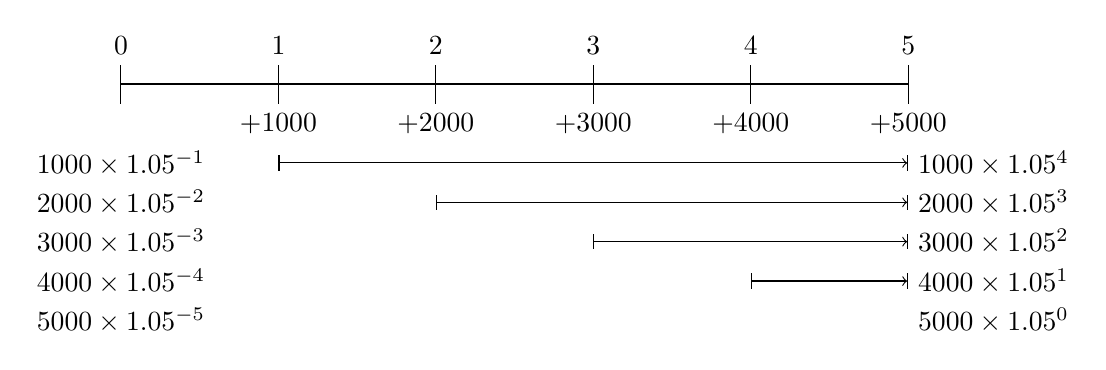
\begin{tikzpicture}
    \draw[thick] (0,0) -- (10,0);
    \foreach \x [count=\k] in {0,...,5}
        {
        \draw[thin] (\x*2, -0.25) -- (\x*2, 0.25);
        \node[above] at (\x*2, 0.25)  {\pgfmathparse{\timf[\k-1]}\pgfmathresult};
        \node[below] at (\x*2, -0.25) {\pgfmathparse{\tvmf[\k-1]}\pgfmathresult};
        }
    \draw (2, -1.0) edge[|->|] (10, -1.0);
    \node[right] at (10, -1.0) {\pgfmathparse{"$1000 \times 1.05^4$"}\pgfmathresult};
    \node at (0, -1.0) {\pgfmathparse{"$1000 \times 1.05^{-1}$"}\pgfmathresult};
    \draw (4, -1.5) edge[|->|] (10, -1.5);
    \node[right] at (10, -1.5) {\pgfmathparse{"$2000 \times 1.05^3$"}\pgfmathresult};
    \node at (0, -1.5) {\pgfmathparse{"$2000 \times 1.05^{-2}$"}\pgfmathresult};
    \draw (6, -2.0) edge[|->|] (10, -2.0);
    \node[right] at (10, -2.0) {\pgfmathparse{"$3000 \times 1.05^2$"}\pgfmathresult};
    \node at (0, -2.0) {\pgfmathparse{"$3000 \times 1.05^{-3}$"}\pgfmathresult};
    \draw (8, -2.5) edge[|->|] (10, -2.5);
    \node[right] at (10, -2.5) {\pgfmathparse{"$4000 \times 1.05^1$"}\pgfmathresult};
    \node at (0, -2.5) {\pgfmathparse{"$4000 \times 1.05^{-4}$"}\pgfmathresult};
    \node[right] at (10, -3.0) {\pgfmathparse{"$5000 \times 1.05^0$"}\pgfmathresult};
    \node at (0, -3.0) {\pgfmathparse{"$5000 \times 1.05^{-5}$"}\pgfmathresult};
\end{tikzpicture}
\end{center}
It is better to use a financial calculator in this case then when it is already programmed to compute this kind of problem quickly. 


\subsection{Types of problems in the CFA examination}
In the CFA exam, the following types of problems related to the TVM can be encountered:
\begin{itemize}
	\setlength\itemsep{0em}
	\item Compute an annuity payment $PMT$ needed to achieve a given $FV$
	\item Compute a loan payment
	\item Compute the required payment to fund an annuity due beginning at time zero or later than that
	\item Compute the number of periods or years in an annuity $N$
	\item Compute the rate of return or discount rates $r (I/Y)$ for an annuity
\end{itemize}



\section{QM - Statistical concepts and Market returns}

\subsection{Fundamental concepts}
Statistics is used to refer to data and the methods we use to analyze data. Statistical methods fall into one of two categories:
\begin{itemize}
	\setlength\itemsep{0em}
	\item \textbf{descriptive statistics} are used to summarize the important characteristics of large data sets;
	\item \textbf{inferential statistics} pertain to forecasts, estimates, or judgments about a large set of data on the basis of the statistical characteristics of a smaller set (a sample).
\end{itemize}

A \textbf{population} is defined as the set of all possible members of a stated group. A sample is defined as a subset of the population of interest. 

Different statistical methods use different levels of measurement, or measurement scales. Measurement scales may be classified into one of four major categories:
\begin{itemize}
	\setlength\itemsep{0em}
	\item \textbf{nominal scales} observations are classified or counted with no particular order.
	\item \textbf{ordinal scales} every observation is assigned to one of several categories.
	\item \textbf{interval scales} provide relative ranking, like ordinal scales, plus the assurance that differences between scale values are equal.
	\item \textbf{ratio scales} provide ranking and equal differences between scale values, and they also have a true zero point as the origin.
\end{itemize}

A measure used to describe a characteristic of a population is referred to as a parameter, e.g. investment analysis usually utilizes just the mean return and the standard deviation of returns.

A sample statistic is used to measure a characteristic of a sample.

A frequency distribution is a tabular presentation of statistical data that aids the analysis of large data sets. A procedure used to construct a frequency distribution can be described as:
\begin{itemize}
	\setlength\itemsep{0em}
	\item define the intervals
	\item tally the observations
	\item count the observations, i.e. the absolute frequency
\end{itemize} 
A histogram is the graphical presentation of the absolute frequency distribution.

The relative frequency is calculated by dividing the absolute frequency of each return interval by the total number of observations. The cumulative absolute frequency and cumulative relative frequency are the sums of the absolute or relative frequencies starting at the lowest interval and progressing through the highest, respectively.



\subsection{Measures of Location}

\subsubsection{Means}
Measures of central tendency identify the center, or average, of a data set. This central point can be used to represent the expected value in the data set. 
\begin{itemize}
	\setlength\itemsep{0em}
	\item the population mean of the population with size $N$
	\begin{equation}
		\nu = \frac{\sum_{i=1}^N X_i}{N}
	\end{equation}
	\item the sample mean of a sample of a population with the sample size $n$
	\begin{equation}
		\bar{X} = \frac{\sum_{i=1}^n X_i}{n}
	\end{equation}
\end{itemize}
The population mean is unique. The sample size mean is used to make \textit{inferences} about the population mean. The population mean and sample mean are both examples of \textbf{arithmetic means}.

The geometric mean is often used when calculating \textit{investment returns over multiple periods} or when measuring \textit{compound growth rates}. The general formula for the geometric mean is as follows:
\begin{equation}
	G = \sqrt[n]{\prod_{i=1}^n X_i}
\end{equation}
However, when calculating the geometric mean for a returns data set, it is necessary to add 1 to each value under the radical and then subtract 1 from the result:
\begin{equation}
	R_G = \sqrt[n]{\prod_{i=1}^n \left( 1 + R_i \right)} - 1
\end{equation}
where $R_i$ is the return for period $i$.

A harmonic mean is used for certain computations, such as the \textit{average cost of shares purchased over time}. The harmonic mean is calculated as:
\begin{equation}
	\bar{X}_H = \frac{N}{\sum_{i=1}^N \frac{1}{X_i}}
\end{equation}

For values that are not all equal: $\bar{X}_H < \bar{X}_G < \bar{X}$. This mathematical fact is the basis for the claimed benefit of purchasing the same dollar amount of mutual fund shares each month or each week. Some refer to this practice as ``dollar cost averaging''.

The computation of a \textbf{weighted mean} recognizes that different observations may have a disproportionate influence on the mean. The weighted mean of a set of numbers is computed as follows:
\begin{equation}
	\bar{X}_w = \sum_{i=1}^n w_i X_i
\end{equation}
where $w_i$ is the weight associated with the observation $X_i$ and $\sum w_i = 1$.
An typical example: the return for a portfolio is the weighted average of the returns of the individual assets in the portfolio. Asset weights are market weights, the market value of each asset relative to the market value of the entire portfolio.

The median is the midpoint of a data set when the data is arranged in ascending or descending order. The median is actually a better measure of central tendency than the mean because it is not affected by extreme values.

The mode is the value that occurs most frequently in a data set. A data set may have one mode (unimodal), more than one mode (bimodal, trimodal...) or even no mode.


\subsubsection{Quantiles}
Quantile is the general term for a value at or below which a stated proportion of the data in a distribution lies. Examples of quantiles include:
\begin{itemize}
	\setlength\itemsep{0em}
	\item Quartiles—the distribution is divided into quarters;
	\item Quintile—the distribution is divided into fifths;
	\item Decile—the distribution is divided into tenths;
	\item Percentile—the distribution is divided into hundredths (percents).
\end{itemize}
The formula for the position of the observation at a given percentile $y$ with $n$ data points sorted in ascending order is:
\begin{equation}
	L_y = (n+1) \frac{y}{100}
\end{equation}


\subsection{Measure of Dispersion}



\subsection{Symmetry, Skewness and Kurtosis in return distributions}



\section{QM - Probability concepts}

\subsection{Fundamental concepts}

\subsection{Portfolio expected return and Variance of return}

\subsection{Probability distributions}

\subsection{Discrete random variables}

\subsection{Continuous random variables}

\subsection{Monte Carlo simulation}


\section{QM - Sampling and Estimation}


\section{QM - Hypothesis testing}

